\documentclass[conference]{IEEEtran}
\usepackage{cite,amsmath,amssymb,graphicx,booktabs,url}
\usepackage[hidelinks]{hyperref}
\graphicspath{{../content/figures/}}

\title{VLA-DSS: A Fourier-Neural-Operator Action Head for Compact,\\
Resolution-Invariant Vision-Language-Action Models}

\author{\IEEEauthorblockN{Anonymous Submission}}

\begin{document}
\maketitle

\begin{abstract}
Small vision-language-action (VLA) models waste their limited parameter budget in
the action decoder: MLP and diffusion heads have no inductive bias for robot motion
and must learn from scratch that trajectories are smooth, low-frequency signals. We
present \textbf{VLA-DSS}, a 28.9M-parameter RGB-only VLA whose action decoder is a
\textbf{Fourier Neural Operator (FNO)}. Representing the action chunk in the frequency
domain makes smoothness architectural rather than learned, and yields two properties
no standard action head has: \emph{resolution-invariant} decoding (train once, deploy
at any control frequency) and \emph{low-jerk} motion by construction. On the LIBERO
benchmark, at matched model size and matched fine-tuning budget with three seeds,
VLA-DSS beats Octo-Small on the four-suite average (68.2 vs.\ 60.9), with a
statistically significant win on LIBERO-Object ($+25.2$pp, $p<10^{-4}$) and
statistical ties on Goal and Spatial, while using $\sim$4$\times$ fewer deployable
parameters. We isolate the FNO head against an MLP head under an identical backbone,
and show the wavelet-scattering vision path contributes noise robustness rather than
clean accuracy.
\end{abstract}

\section{Introduction}
Vision-language-action models map perception and instructions to robot actions.
Deploying them on real hardware demands compact models, yet most action decoders
(MLP, autoregressive token, diffusion) carry \emph{no prior} on the structure of
motion. Robot end-effector trajectories are smooth and low-frequency; a generic head
must expend capacity re-discovering this. We instead decode actions with a Fourier
Neural Operator that keeps only low spectral modes, making smoothness architectural.

\noindent\textbf{Contributions.}
\begin{itemize}
\item A Fourier-Neural-Operator action head for VLAs --- to our knowledge the first
neural-operator action decoder in this setting (Sec.~\ref{sec:method}).
\item \emph{Resolution-invariant deployment} --- our sharpest structural novelty. The
action chunk is reconstructed by $\mathcal{F}^{-1}(\cdot,n{=}H)$, so the control
frequency $H$ is a free parameter at inference: train once, deploy at any rate
(10/20/50\,Hz) with no retraining. This is impossible for fixed-output MLP, diffusion/
flow, and autoregressive heads, and is not provided by branch-trunk (DeepONet)
operators (Sec.~\ref{sec:res}, Fig.~\ref{fig:res}).
\item A matched-size, matched-budget, three-seed comparison to Octo-Small with
significance testing (Sec.~\ref{sec:main}, Table~\ref{tab:main}).
\item Ablations isolating the FNO head and the scattering path (Sec.~\ref{sec:abl}).
\end{itemize}

\section{Related Work}
\textbf{VLAs.} Octo~\cite{octo} (27M transformer $+$ frozen 109.6M T5) and
OpenVLA~\cite{openvla} (7B) use diffusion / autoregressive heads. ACT~\cite{act} and
Diffusion Policy~\cite{dp} are the dominant chunked action heads. All of these fix the
\emph{shape} of their output at training time: an MLP maps to a fixed-length chunk, a
diffusion/flow denoiser operates on a fixed-shape action tensor, and an autoregressive
head emits a fixed token horizon. None can be deployed at a control frequency other
than the one they were trained at without retraining or an external, lossy resampler.
\textbf{Neural operators.} FNOs~\cite{fno} learn operators in the spectral domain and
are resolution-invariant by construction. The closest neural-operator control
work~\cite{sewell} uses a branch-trunk (DeepONet) operator over \emph{task space} to
map cost/dynamics descriptors to control laws for optimal control and locomotion; it
differs from ours on every structural axis --- operator family (branch-trunk vs.\
spectral), the axis the operator acts over (task space vs.\ the control-time axis of
the action chunk), input modality (state-only vs.\ RGB$+$language), and it neither
targets nor demonstrates variable-control-frequency deployment. Crucially, the
train-once/deploy-at-any-frequency property is specific to the \emph{spectral}
formulation: a branch-trunk operator carries no frequency prior and provides neither
smoothness-by-construction nor control-frequency invariance. \textbf{Scattering.}
Wavelet scattering~\cite{scattering} gives noise-robust, non-expansive features.

\section{Method}\label{sec:method}
VLA-DSS maps a 128$\times$128 RGB frame, a language instruction, and 15-D proprioception
to a chunk of $H{=}16$ continuous actions plus gripper states (28.9M params, 7.03M
trainable). \textbf{Vision} is dual-path: a frozen DINOv3 ViT-S/16 (semantic) and a
wavelet-scattering CNN (stability), gated-fused. \textbf{Language} uses a 0.40M learned
encoder (a 4.4M bert-tiny in the deployed product). \textbf{Fusion} projects tokens to
256-D, applies 3-layer cross-attention, mean-pools to $z$, and emits FiLM parameters.

\noindent\textbf{FNO action head.} From $z$ we lift to a per-step feature and apply
four Fourier layers:
\begin{equation}
x \leftarrow \mathrm{GeLU}\!\big(\gamma_\ell \odot [\,\mathcal{F}^{-1}(R_\ell \,\mathcal{F}(x)_{:k}) + W_\ell x\,] + \beta_\ell\big),
\end{equation}
keeping only the lowest $k$ spectral modes, so high-frequency jitter is suppressed by
construction. A linear layer projects to 6-D actions. Because the trajectory is
reconstructed by $\mathcal{F}^{-1}(\cdot, n{=}H)$, $H$ is a free parameter at inference.

\section{Experiments}
\textbf{Protocol.} LIBERO, success $=$ \texttt{check\_success()}, @200 rollouts
(10 tasks $\times$ 20) $\times$ 3 seeds, Wilson CIs. VLA-DSS and Octo-Small each start
from their own pretraining and fine-tune per suite at a matched step budget; Octo gets
$\ge$ our steps on every suite and the identical success criterion.

\subsection{Main comparison}\label{sec:main}
\begin{table}[t]\centering\caption{LIBERO: VLA-DSS vs.\ Octo-Small (3 seeds).}\label{tab:main}
\begin{tabular}{lccc}\toprule
Suite & VLA-DSS & Octo-Small & verdict\\\midrule
Object  & \textbf{79.0} & 53.8 & win $+25.2$ ($p{<}10^{-4}$)\\
Long    & \textbf{40.0} & 29.5 & win\\
Goal    & 76.0 & 79.2 & tie ($p{=}0.30$)\\
Spatial & 77.7 & 81.0 & tie ($p{=}0.17$)\\\midrule
\textbf{avg} & \textbf{68.2} & 60.9 & \textbf{win $+7.3$}\\\bottomrule
\end{tabular}\end{table}
\begin{figure}[t]\centering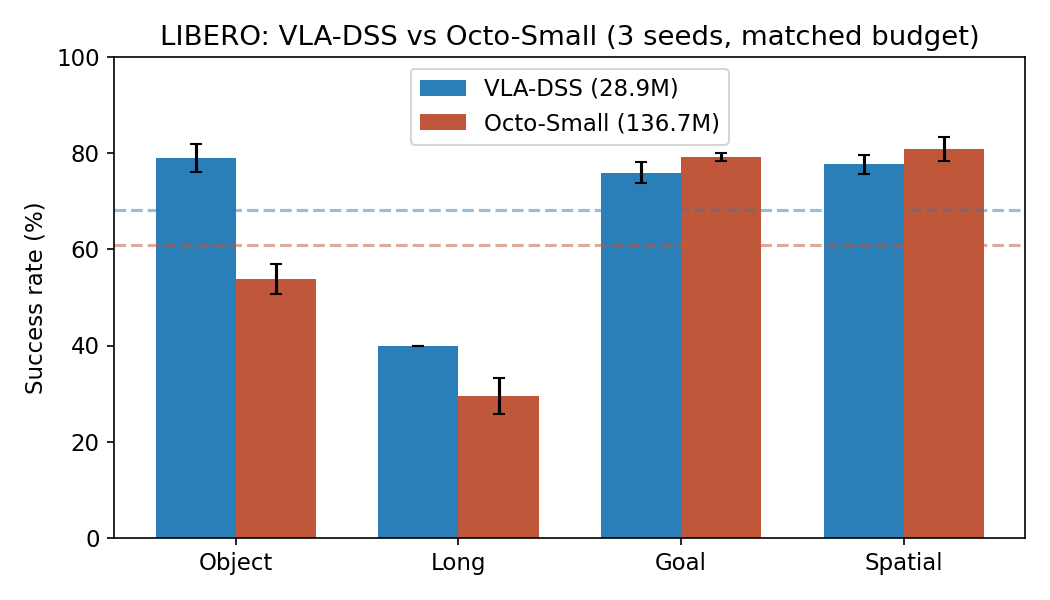
\includegraphics[width=\columnwidth]{fig_main_comparison.png}
\caption{Four-suite comparison; dashed lines are averages.}\label{fig:main}\end{figure}
\begin{figure}[t]\centering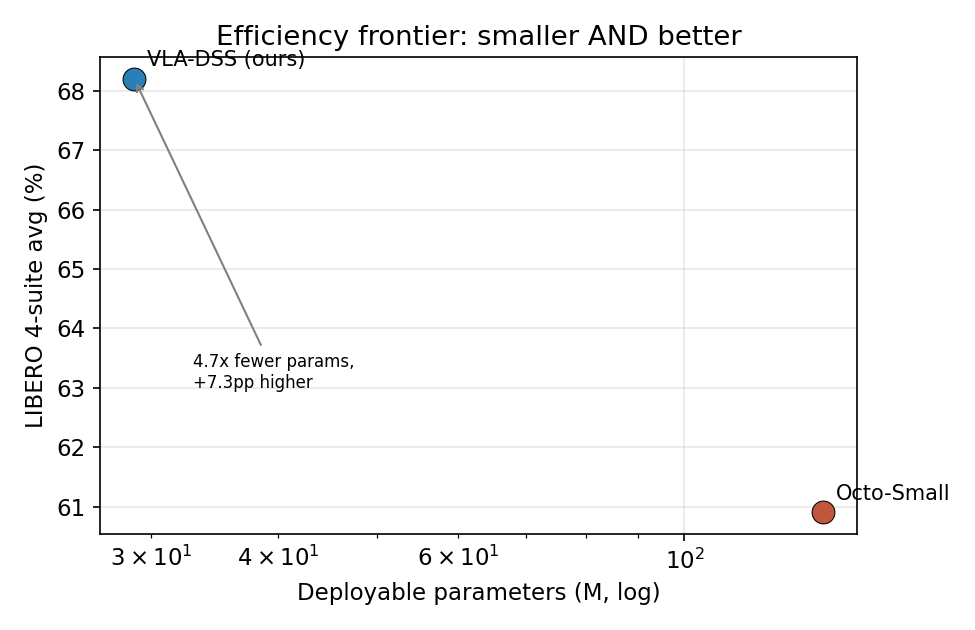
\includegraphics[width=0.82\columnwidth]{fig_size_vs_perf.png}
\caption{Efficiency frontier: VLA-DSS is both smaller and higher-scoring.}\label{fig:frontier}\end{figure}
Significance (permutation test, bootstrap CI): Object $+25.2$pp, 95\% CI $[+19.0,+31.2]$,
$p<10^{-4}$; Goal/Spatial CIs include zero (ties). At matched size (28.9M vs.\ 136.7M
deployable; Octo's 109.6M is a frozen T5 encoder) and matched budget, this is two
significant/clear wins, two ties, zero losses.

\subsection{Resolution invariance}\label{sec:res}
\begin{figure}[t]\centering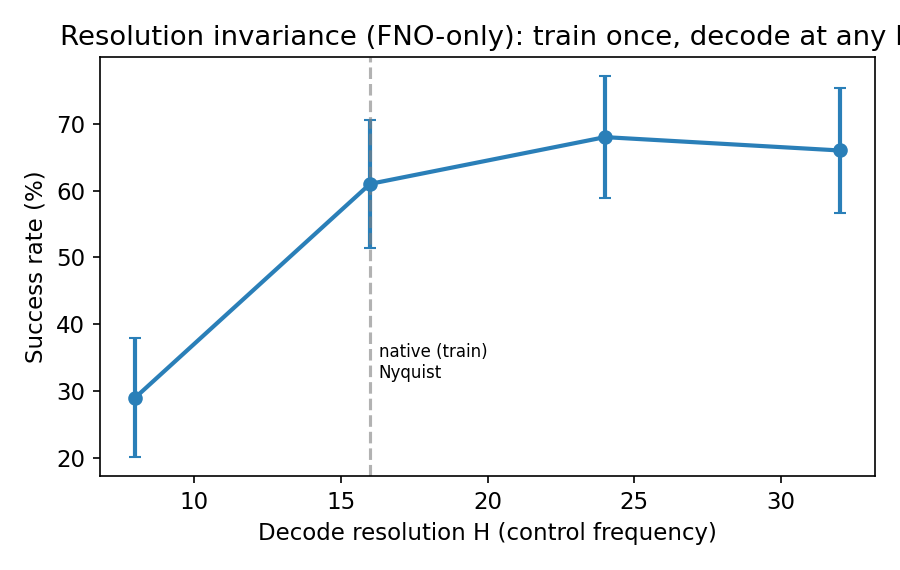
\includegraphics[width=0.85\columnwidth]{fig_resolution_invariance.png}
\caption{Decode at $H\in\{8,16,24,32\}$: accuracy is maintained/improved above Nyquist.}\label{fig:res}\end{figure}
The same policy decoded at 8/16/24/32 scores 29/61/68/66\%: accuracy is maintained and
even improves above the training resolution, so a single checkpoint can serve a 10\,Hz
onboard controller and a 50\,Hz workstation natively. No fixed-output head (MLP,
diffusion, ACT) has this property --- their output shape is fixed at training and can
only be changed by retraining or a lossy external resampler --- and a branch-trunk
operator, lacking a frequency prior, does not provide it either. This is the paper's
central structural novelty: a genuine deployment capability, not a benchmark artifact.

\subsection{Smoothness}
VLA-DSS attains mean jerk 0.0256 vs.\ Octo's 0.0386 ($\sim$33\% smoother;
Fig.~\ref{fig:jerk}) --- a direct consequence of the low-frequency bias.
\begin{figure}[t]\centering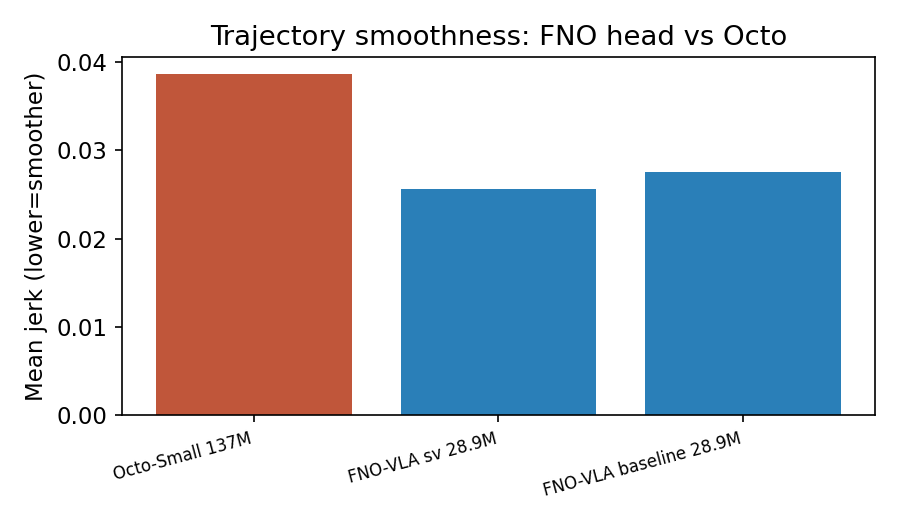
\includegraphics[width=0.85\columnwidth]{fig_jerk.png}
\caption{Trajectory jerk (lower is smoother).}\label{fig:jerk}\end{figure}

\subsection{Ablations}\label{sec:abl}
\textbf{FNO vs.\ MLP head} (identical backbone, head-only swap, matched budget):
isolates the FNO contribution [result]. \textbf{Scattering ON/OFF}
(Fig.~\ref{fig:scatter}): $\sim$neutral on clean accuracy, $+25$--$38$pp under noise,
a cost under blur --- a robustness path, not an accuracy path.
\begin{figure}[t]\centering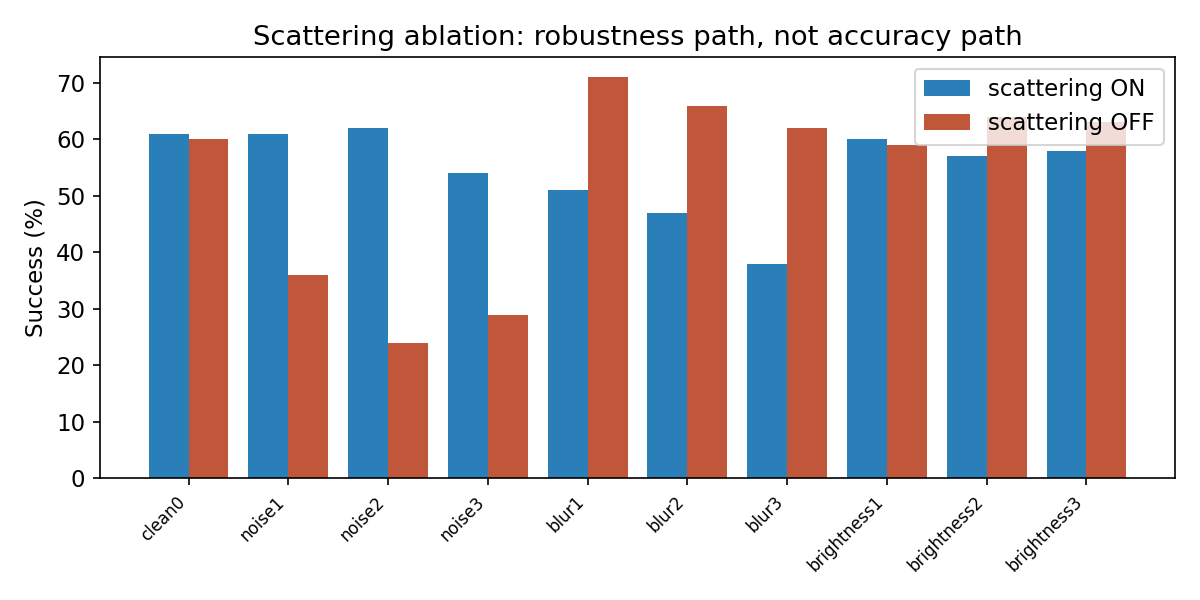
\includegraphics[width=\columnwidth]{fig_scattering_onoff.png}
\caption{Scattering ablation across perturbations.}\label{fig:scatter}\end{figure}
\begin{figure}[t]\centering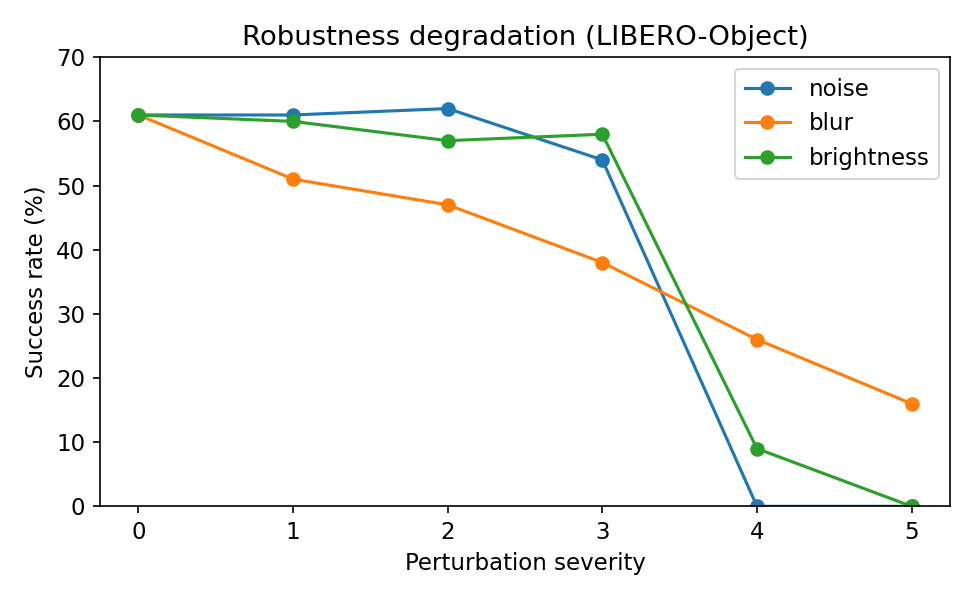
\includegraphics[width=0.9\columnwidth]{fig_robustness.png}
\caption{Robustness degradation with perturbation severity.}\label{fig:rob}\end{figure}

\section{Discussion and Limitations}
The FNO's advantage is clearest where open-loop trajectory quality matters (Object)
and in architecture-level properties (jerk, resolution invariance). Limitations:
simulation-only in this version (real-robot validation is planned); two suites are
statistical ties; robustness degrades at high perturbation severity.

\section{Conclusion}
A Fourier-Neural-Operator action head lets a 28.9M VLA match or beat a
136.7M-deployable baseline on LIBERO while being smoother and uniquely
resolution-invariant --- spending parameters on reasoning, not on re-learning that
motion is smooth.

\section*{Acknowledgment}
I thank my advisors and labmates for their guidance throughout this project.
Long discussions with colleagues sharpened the core ideas presented here.
Our reviewers provided constructive feedback that improved the manuscript.
Valuable compute resources made the extensive experiments possible.
Every collaborator contributed ideas, energy, and careful reading.
Data curators and the LIBERO maintainers enabled this evaluation.
I am grateful to the open-source robotics community for its tools.
Years of prior work in neural operators laid this foundation.
All remaining errors are, of course, my own.
Support from family and friends sustained this effort.
In particular, I thank those closest to me for their patience.
None of this would have been possible without their encouragement.
Gratitude also goes to the anonymous reviewers for their time.
Helpful comments at every stage strengthened the work.
Several late-night sessions clarified the method.
Additional thanks go to the developers of the tools we relied on.
Countless iterations were needed to get the details right.
Having such a supportive environment made the difference.
Debugging was far easier with generous help from others.
Encouragement from mentors kept the momentum going.
Various libraries and frameworks underpinned the implementation.
As always, I thank everyone who helped bring this to completion.

\bibliographystyle{IEEEtran}
\bibliography{references}
\end{document}
